\chapter{Surfaces}
\label{sec:surfaces}


A \myindx{surface} can be created as a function of two variables $z=f(x,y)$ analogous to the curves described earlier.
However this representation suffers from the same problems, namely that only simple geometries can 
be described. In stead we will move directly to the parametric description of surfaces.

A surface can be parametrized by two parameters u,v. 

$$
  \vec{r} = (x,y,z) = \Big( x(u,v),y(u,v),z(u,v) \Big)
$$

This representation is much more flexible: $x,y$ and $z$ are free to move in 
arbitrarily complicates ways to create closed and convoluted surfaces. One example
is shown on the front page. This is a surface folded like a \myindx{trefoil knot}.

\section{Sphere}

In order to create a 2D surface we must place some restrictions on the three coordinates.
For example by fixing r to $r_0$ and
letting $\theta$ and $\phi$ run through their allowed ranges produces a sphere, and
we say that the surface is parametrized by the two coordinates $\theta$ and $\phi$.

$$
  \vec{r}(\theta,\phi) = r_0(\stsp, \stcp, \ct)
$$

$$
   \vec{e}_1 = 
    \vec{e}_\theta = 
    \dvd{r}{\theta} = 
    \vc{\ctsp}{\ctcp}{-\st}
$$

$$
   \vec{e}_2 = \vec{e}_\phi = \dvd{r}{\phi} = \vc{\stcp}{-\stsp}{0}
$$

\index{metric tensor!sphere}
$$
    g_{ij} = \vec{e}_i\cdot\vec{e}_j = \left( \begin{array}{ccc}
      1 & 0 \\
      0 & \sin^2\theta
    \end{array} \right)
$$


\begin{figure}[!ht]
  \begin{center}
    \begin{pspicture}(-4,-4)(4,4) 
    \psset{unit=3cm}
      \pstThreeDCoor[xMin=-1.5,xMax=1.5, yMax=1.5, zMax=1.5] 
      \pstThreeDSphere[SegmentColor={[cmyk]{0,0,0,0}}](0,0,0){1} 
      \parametricplotThreeD[algebraic,plotstyle=curve,linewidth=1.5pt](0,3.1415)
          {0| sin(t)|cos(t)}
    \end{pspicture}
  \end{center}
  \caption{\small Sphere with a curve going from north to south along a \myindx{great circle}.}
  \label{fig-sph_geo}
\end{figure}

\section{Curves on a sphere}

Let us now describe curves on a surface. A curve can be parametrized by a single parameter, t. This looks as follows in the case of spherical coordinates (note that r is constant)

$$
  \vec{r}(t) = r_0\Big(\sin\Big(\theta(t)\Big) \cos\Big(\phi(t)\Big), \sin\Big(\theta(t)\Big)\sin\Big(\phi(t)\Big), \cos\Big(\theta(t)\Big)\Big)
$$

Letting $\phi(t)=0$, $\theta(t)=t$ and $ 0\le t \le \pi$ gives the following simple curve:

$$
  \vec{r}(t) = r_0(\sin(t), 0, \cos(t))
$$


This is a great circle from the north pole to the south pole. The length of this curve is simply $\pi r_0$.

By chosing the following parametrization $\theta(t)=t,\quad \phi(t)=2t-\pi$ we obtain the following cute winding curve shown in figure \ref{fig-sph_wind}


\begin{figure}[!ht]
  \begin{center}
    \begin{pspicture}(-4,-4)(4,4) 
    \psset{unit=3cm}
      \pstThreeDCoor[RotZ=90,xMin=-1.5,xMax=1.5, yMax=1.5, zMax=1.5] 
      \pstThreeDSphere[SegmentColor={[cmyk]{0,0,0,0}}](0,0,0){1} 
      \parametricplotThreeD[algebraic,plotstyle=curve,linewidth=1.5pt](0,2)
          {sin(t)*cos(2*t-3.1415)| sin(t)*sin(2*t-3.1415)|cos(t)}
      \parametricplotThreeD[algebraic,plotstyle=curve,linestyle=dashed,linewidth=1.5pt](2,3.1415)
          {sin(t)*cos(2*t-3.1415)| sin(t)*sin(2*t-3.1415)|cos(t)}
    \end{pspicture}
  \end{center}
  \caption{\small Sphere with a curve winding down from north to south.}
  \label{fig-sph_wind}
\end{figure}

$$
   l = r_0\int_0^\pi{\sqrt{g_{11}\dot{\theta}^2 + g_{22}\dot{\phi}^2 }}dt = r_0\int_0^\pi{\sqrt{1+4\sin^2t}}dt \approx r_0\cdot5.27037\ldots
$$


\section{Cylinder}

We can parametrize the \myindx{cylinder} by $\theta$ and $z$ by setting $\rho=\rho_0$,

$$ \vec{r}(\theta,z) = (\rho_0\st, \rho_0\ct, z) $$


$$ \vec{e}_1=\vec{e}_\theta =\dvd{r}{\theta} = \var{\rho_0\ct}{-\rho_0\st}{0} $$

$$ \vec{e}_2=\vec{e}_z =\dvd{r}{z} = \var{0}{0}{1}
$$

\index{metric tensor!cylinder}
$$
   g_{ij} =\vec{e}_i\cdot\vec{e}_j=  \left( \begin{array}{cc}
                    \rho_0^2 & 0 \\
                    0      & 1 
                    \end{array} 
             \right)
$$

Since the metric tensor for the cylinder surface is constant the surface has zero \myindx{curvature}. 

\begin{figure}[!ht]
  \begin{center}
    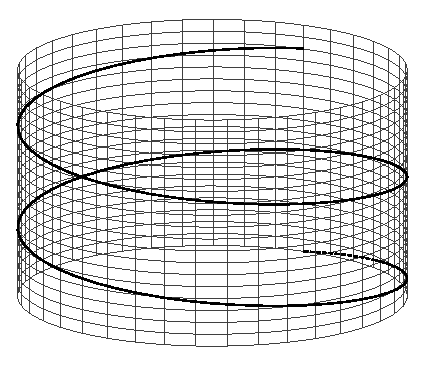
\includegraphics[width=6cm,height=6cm]{figures/cyl}
  \end{center}

  \caption{\small Cylinder surface with a spiral curve.}
  \label{fig-cyl}
\end{figure}

\section{Curves on a cylinder}
We parametrize a curve on the cylinder by letting $\rho,\theta,z$ depend on a single parameter, and thus get the coordinates as a function of $t$.

$$ \vec{r}(t) = (\rho_0\st(t), \rho_0\ct(t), z(t))$$

If we let $\theta(t)=bt$, nd $z(t)=at$, where we can think of $b$ as the rotation speed and $a$ as the speed along the $z$ axis, we obtain

$$ \vec{r}(t) = (\rho_0\sin(bt), \rho_0\cos(bt), at) $$ 
which, with $a=1, b=2$, gives the curve shown in figure \ref{fig-cyl}. The length of this curve is

$$
   l = \int_0^{2\pi}{\sqrt{g_{11}\dot{\theta}^2 + g_{22}\dot{z}^2 }}dt = \int_0^{2\pi}{\sqrt{ b^2\rho_0^2  + a^2 }}dt = 2\pi\sqrt{a^2+b^2\rho_0^2} 
$$

This seems reasonable: When $a=0$ the curve degenerates to a circle with the radius $\rho_0$, and the length is simply the length of the circle, $2\pi\rho_0$, times the number of windings $b$.

\section{Paraboloid}
A well known surface is the \myindx{paraboloid}, which is the same shape as a \myindx{satellite disk}. Its parametrization is
$$
   \vec{r}(u,v) = (u, v, -(u^2 +v^2))
$$

$$
   \vec{e}_1 = \vec{e}_u = \dvd{r}{u} = \left( \begin{array}{c} 
        1 \\
        0 \\
        -2u 
   \end{array} \right)
$$

$$
   \vec{e}_2 = \vec{e}_v = \dvd{r}{v} = \left( \begin{array}{c} 
        0 \\
        1 \\
        -2v 
   \end{array} \right)
$$

\index{metric tensor!paraboloid}
$$
    g_{ij} = \vec{e}_i\cdot\vec{e}_j = \left( \begin{array}{ccc}
      1 +4u^2 & 4uv \\
      4uv & 1 + 4v^2 
    \end{array} \right)
$$
This is the first case where $g_{12}=g_{21}$ is not zero.

\begin{figure}[!ht]
  \begin{center}
    \psset{unit=0.75} 
    \begin{pspicture}(-5.5,-6)(4.5,4) 
      \psset[pst-solides3d]{viewpoint=35 -60 80 rtp2xyz, Decran=50,lightsrc=viewpoint} 
      % Parametric Surfaces
      \defFunction[algebraic]{hyppar}(u,v) 
          {u} {v} {-(u*u + v*v) }
      \defFunction{hypline}(t) 
          {t t Sin mul} {t t Cos mul} { t t mul t Sin t Sin mul t Cos t Cos mul add mul neg }
      \psSolid[object=surfaceparametree, action=draw*, linecolor=black!75,linewidth=0.01, 
          base=pi neg pi pi  neg  pi, fillcolor=blue!20,incolor=black!20, function=hyppar,
          linewidth=0.5 \pslinewidth,ngrid=25]
      \psSolid[object=courbe, r=0, range= pi  neg pi , action=draw*, linecolor=black, 
               linewidth=0.05,resolution=360, function=hypline]
    \end{pspicture}
  \end{center}

  \caption{\small Paraboloid surface.}
  \label{fig-parab}
\end{figure}


\section{Curves on the paraboloid}
The curve on the paraboloid surface shown in figure \ref{fig-parab} is parametrized as
$$
u(t)=t\sin(t),\quad v(t)=t\cos(t), \quad -\pi\le t \le\pi
$$

\begin{align}
   f(t) &= g_{11}\dot{u}^2 +2g_{12}\dot{u}\dot{v}+ g_{22}\dot{v}^2 \notag\\
             &=(1+4t^2\sin^2t)(\sin(t) + t\cos(t))^2\notag\\
             &+ 8t^2\sin(t)\cos(t)(\cos(t) - t\sin(t)) (\sin(t) + t\cos(t))\notag\\
             &+ (1+4t^2\cos^2t)(\cos(t) - t\sin(t))^2 \notag
\end{align}

 and the length of the curve is 

$$
  = \int_{-\pi}^{\pi}{\sqrt{ f(t) }}dt \approx 23.47564\ldots
$$


\section{Hyperbolic paraboloid}
The \myindx{hyperbolic paraboloid} is a surface, shown in figure \ref{fig-hyp_curv}, which can be parametrized by u,v in the following manner
$$
   \vec{r}(u,v) = (u, v, u^2 -v^2)
$$



\begin{figure}[!ht]
  \begin{center}
    \psset{unit=0.75} 
    \begin{pspicture}(-5.5,-6)(4.5,4) 
      \psset[pst-solides3d]{viewpoint=45 210 50 rtp2xyz, Decran=50,lightsrc=45 -50 330} 
      % Parametric Surfaces
      \defFunction[algebraic]{hyppar}(u,v) 
          {u} {v} {(u*u - v*v)/4 }
      \defFunction{hypline}(t) 
          {t t Sin mul} 
          {t t Cos mul} 
          { t t mul t Sin t Sin mul t Cos t Cos mul sub mul 4 div }
      \psSolid[object=surfaceparametree, action=draw*, linecolor=black!75,linewidth=0.01, 
          base=pi neg pi pi  neg  pi, 
          fillcolor=blue!20,incolor=black!20, function=hyppar,linewidth=0.5 \pslinewidth,ngrid=25]
      \psSolid[object=courbe, r=0, range= pi  neg pi , action=draw*, linecolor=black, 
               linewidth=0.05,resolution=360, function=hypline]
    \end{pspicture}
  \end{center}

  \caption{\small Hyperbolic paraboloid surface.}
  \label{fig-hyp_curv}
\end{figure}




$$
   \vec{e}_1 = \vec{e}_u = \dvd{r}{u} = \left( \begin{array}{c} 
        1 \\
        0 \\
        2u 
   \end{array} \right)
$$

$$
   \vec{e}_2 = \vec{e}_v = \dvd{r}{v} = \left( \begin{array}{c} 
        0 \\
        1 \\
        -2v 
   \end{array} \right)
$$

\index{metric tensor!hyperbolic paraboloid}
$$
    g_{ij} = \vec{e}_i\cdot\vec{e}_j = \left( \begin{array}{ccc}
      1 +4u^2 & -4uv \\
      -4uv & 1 + 4v^2 
    \end{array} \right)
$$

The metric tensor is similar to the one for the paraboloid surface, differing only
in the sign of the cross terms.




\section{Curves on the hyperbolic paraboloid}
The curve shown in figure \ref{fig-hyp_curv} is created by the same parametrization as 
for the paraboloid in figure \ref{fig-parab}.
$$
u(t)=t\sin(t),\quad v(t)=t\cos(t),\quad -\pi\le t \le \pi
$$

\begin{align}
   g(t) &= g_{11}\dot{u}^2 +2g_{12}\dot{u}\dot{v}+ g_{22}\dot{v}^2 \notag\\
             &=(1+4t^2\sin^2t)(\sin(t) + t\cos(t))^2\notag\\
             &- 8t^2\sin(t)\cos(t)(\cos(t) - t\sin(t)) (\sin(t) + t\cos(t))\notag\\
             &+ (1+4t^2\cos^2t)(\cos(t) - t\sin(t))^2 \notag
\end{align}

 and the length of the curve is 

$$
  = \int_{-\pi}^{\pi}{\sqrt{ g(t) }}dt \approx 35.57158\ldots
$$


\newcommand{\sh}{a\sin\omega\theta + b} 
\section{Modulated sphere}
A slightly more complicated surface can be created by allowing r to depend on $\theta$ and $\phi$,
For example as $r(\theta,\phi) = \sh$. When $a=0.1, \omega=10, b=1$, the result is the following parametrization of the ``modulated sphere'' shown in figure \ref{fig-def_sph_wind}

\newcommand{\rtp}{r(\theta,\phi)}
$$
  \vec{r}(\theta,\phi) = (\rtp\stsp, \rtp\stcp, \rtp\st)
$$

\begin{figure}[!ht]
  \begin{center}
    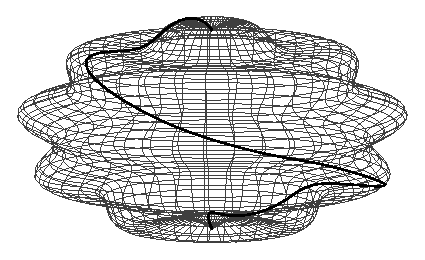
\includegraphics[width=6cm,height=6cm]{figures/def_sph_wind}
  \end{center}

  \caption{\small Modulated sphere ($a=0.1, \omega=10, b=1$)}
  \label{fig-def_sph_wind}
\end{figure}

Now it gets a little complicated..

$$
    \vec{e}_1=\vec{e}_\theta=\dvd{r}{\theta} = 
        \left( \begin{array}{c}
          \left[a\ct\sin(\omega\theta)+a\omega\st\cos(\omega\theta)+b\ct\right] \sip \\ 
          \left[a\ct\sin(\omega\theta)+a\omega\st\cos(\omega\theta)+b\ct\right] \cop \\ 
               -a\st\sin(\omega\theta)+a\omega\ct\cos(\omega\theta)-b\st
        \end{array} \right)
$$

$$
    \vec{e}_2=\vec{e}_\phi=\dvd{r}{\phi} = 
        \left( \begin{array}{c}
         (\sh)\stcp\\ 
         - (\sh)\stsp\\ 
            0
        \end{array} \right)
$$

..and after some manipulations, where we primarily use the \myindx{trigonometric identity} \mbox{$\sin^2a + \cos^2a = 1$}, we get 


$$
    g_{ij} = \vec{e}_i\cdot\vec{e}_j = \left( \begin{array}{ccc}
      f(\theta) & 0 \\
      0  & (\sh)^2\sin^2\theta 
    \end{array} \right)
$$
Where

\begin{align}
 f(\theta) & =   \Big((a\sin(\omega\theta)+b)\ct +a\omega\st\cos(\omega\theta)\Big)^2  \notag\\ 
          & + \Big(-(a\sin(\omega\theta)+b)\st+a\omega\ct\cos(\omega\theta)\Big)^2 \notag\\
          &= (\sh)^2  + a^2\omega^2\cos^2(\omega\theta)\notag 
\end{align}

Note that already at this stage the formulae gets so complicated that there is great risk in not 
getting it right by hand calculation, and no chance of analytic integration. But we can check that 
this is plausible by noting that in the limit of no deformation $(a,b)\to (0,1)$, $f=1$ and we 
recover the metric tensor for the sphere.

\section{Curves on the modulated sphere}
Using the same parametrization, $\theta(t)=t, \phi(t)=2t-\pi$, as for the winding curve on the sphere we get a complicated curve as shown in figure \ref{fig-def_sph_wind}. Since
$$
   g_{11}\dot{\theta}^2 + g_{22}\dot{\phi}^2 = f(t) + 4(a\sin\omega t + b)^2\sin^2t
$$
we obtain the formula for the curve length as 

$$
   l = \int_0^\pi{\sqrt{ f(t) + 4(a\sin\omega t + b)^2\sin^2t }}dt \approx 5.73653\ldots
$$




